% \section{État au commencement du projet}
Le projet etant open-source et actif, il evolue sans cesse. La partie sur laquelle nous avons travaille est relativement stable mais son utilisation peut varier dans le code. Nous allons voir la portee de l'utilisation de nanoXml, comment il est utilise et enfin la solution apportee.

% -> Utilisation intensive de XML
% -> Philosophie de nanoXml et de DOM differente
% -> -> DOM : Tout est noeud
% -> -> NanoXml : Base sur les tags (elements)
\section{Nanoxml}
Comme nous avons pu le voir, IzPack utilise intensemment des fichiers XML pour gerer la generation d'installations. En effet, les fichiers XML presentent l'avantage d'etre lisible, ecrivable a la main et traitables. Pour traiter ces fichiers, une librairie a ete utilisee, il s'agit de NanoXml.
\subsection{Le projet NanoXml}
NanoXml est une librairie java open-source de gestion de Xml. Elle presente la particularite d'etre legere (108Ko). Il est possible, grace a cette librairie, d'ecrire ou de parser des fichiers Xml. Une fois le fichier parse, on recupere en memoire la structure de l'arbre Xml qui peut alors etre exploite. Le choix de cette librairie a ete fait au commencement de Izpack a cause de sa taille. En effet, il est important que le la partie installeur ne prenne pas le pas sur le logiciel a installer.

Cependant ce projet n'est plus mis a jour depuis 7 ans, et des bugs ont ete decouverts. Entre temps, java a ajoute a sa JRE (depuis la version 1.4) tout ce qu'il faut pour gerer le xml. Il devenait interessant de remplacer NanoXml par Jaxp (Java API for XML Processing), la librairie fournie par la machine virtuelle.
\subsection{Les differents composants de NanoXml}
On trouve differents elements dans NanoXml.
\subsubsection{StdXMLParser}
Le parser permet de creer un arbre logique representant le fichier xml qui lui a ete passe. Il est systematiquement utilise au moment de la lecture du fichier afin de recuperer l'arbre.
\subsubsection{XMLElement}
Le XMLElement represente un element logique du xml en memoire. Par exemple :
\begin{lstlisting}[language=xml]
<root>
	<child>
		content
	</child>
</root>
\end{lstlisting}
En parsant un fichier contenant ce Xml, on a un XMLElement nomme root qui possede 1 enfant, \verb|child|. Son enfant est un XMLElement dont le contenu est content.

L'arborescence du XML est donc realise par un ensemble de XMLElement. XMLElement permet de recuperer la liste des enfants, le contenu, rechercher un enfant par son nom, retirer un enfant, ajouter un enfant ou modifier le contenu. Il s'agit de loin de la classe la plus utilisee de la librairie NanoXml dans Izpack. En effet, on ne comptait pas moins de 499 utilisations au commencement de ce projet.
\subsubsection{StdXMLWriter}
Le XMLWriter permet d'ecrire des fichiers XML. Il reproduit, a partir d'un XML element, le fichier XML correspondant. Il n'est utilise que pour generer un xml temporaire ou pour ecrire le xml d'installation automatique. 
\subsection{Utilisation typique dans Izpack}
\subsubsection{Parse de fichier}
Le parse du fichier est execute pour recuperer le XML.
\begin{lstlisting}
StdXMLParser parser = new StdXMLParser();
parser.setBuilder(XMLBuilderFactory.createXMLBuilder());
parser.setReader(new StdXMLReader(in));
parser.setValidator(new NonValidator());

// We get the data
XMLElement data = (XMLElement) parser.parse();
\end{lstlisting}
Avec cet exemple, on cree les objets necessaires au parse d'un fichier, et on recupere dans data l'element racine du xml.

\subsubsection{Ecriture d'un xml}
\begin{lstlisting}
XMLWriter writer = new XMLWriter(out);
...
writer.write(xmlElement);
\end{lstlisting}
Pour ecrire un xml represente par l'arbre DOM dans xmlElement, il suffit de le passer a un XMLWriter.

\subsubsection{Utilisation de XMLElement}
La manipulation d'un XMLElement se fait avec ses methodes :
\begin{itemize}
	\item get/setAttribute pour gerer les attributs du noeud
	\item get/setContent pour gerer le contenu
	\item add/removeChild pour gerer les noeuds fils
	\item etc
\end{itemize}

Voici un exemple d'utilisation :
\begin{lstlisting}
XMLElement el;
//...
String id = elt.getAttribute("id");
String packImgId = el.getAttribute("packImgId");
boolean loose = "true".equalsIgnoreCase(el.getAttribute("loose", "false"));
String description = requireChildNamed(el, "description").getContent();
boolean required = requireYesNoAttribute(el, "required");
String group = el.getAttribute("group");
String installGroups = el.getAttribute("installGroups");
String excludeGroup = el.getAttribute("excludeGroup");
boolean uninstall = "yes".equalsIgnoreCase(el.getAttribute("uninstall", "yes"));
String parent = el.getAttribute("parent");
String conditionid = el.getAttribute("condition");
\end{lstlisting}
\section{Jaxp}
Jaxp, le processor Xml de Sun, respecte les normes W3C. Il y a deux manieres d'exploiter les XML avec Jaxp, soit en utilisant le parseur Sax, soit en utilisant le parseur DOM.
\subsection{SAX}
SAX (Simple API for Xml) est une API pour parser les XML. Cette API possede la particularite de proceder par evenement. C'est a dire que le parser va lire le fichier ligne par ligne et envoye un evenement pour chaque element particulier qu'il rencontre. 

On a des evenements de commentaires, de text ou d'elements. L'avantages de cette API est l'utilisation memoire faible, puisque le xml n'est pas mis en memoire mais lu et traite au fur et a mesure. Il permet de traiter sans probleme les fichiers importants. En contrepartie, le traitement et la manipulation d'un xml est plus difficile.
\subsection{DOM}
L'interface DOM(Document Object Model) de jaxp propose de mettre en memoire le xml et offre une interaction basee sur des noeuds (node en anglais). En DOM, tout est noeud, et le xml est equivalent a un arbre de noeuds. Les commentaires, le texte ou les elements sont representes par des noeuds. Des sous-classes specialisent ces noeuds. comme \verb|Comment|, \verb|Element| ou \verb|Text|.

La manipulation des elements du xml se fait grace aux nodes. Il est possible de recuperer le voisin d'une node, d'enlever ou d'ajouter un enfant et de recuperer ou de modifier le contenu.
%--------------------------------------------------------------------------
\section{Elaboration de la solution}
Notre travail a ete de chercher une solution pour permettre de remplacer de NanoXml et de l'appliquer au projet. Mais ils y avaient plusieurs problemes a cela.
\subsection{Les differences entre Jaxp et NanoXml}
Comme nous avons vu precedement, les deux API ne proposent pas la meme approche pour le traitement des Xml. Nous avons choisies d'utiliser l'interface DOM vu que les avantages de SAX ne sont pas necessaires et qu'il etait peu concevable de traiter les XML avec SAX dans IzPack. De plus, NanoXml et DOM ont une representation similaire du xml.

Nous allons donc comparer l'interface DOM et NanoXml pour determiner la meilleure approche a prendre.
\subsubsection{Parse du XML}

\subsubsection{Manipulation du XML}
La principale difference vient de l'element atomique : le noeud de DOM ne represente pas la meme notion que l'element de nanoXML. Des lors, la manipulation des voisins, enfants, etc doit etre adapte.
\begin{lstlisting}[language=xml]
<!-- commentaire -->
<root>
	<noeud1>text</noeud1>
</root>
\end{lstlisting}
Dans ce morceau de xml, nanoXML comptera 1 enfant a l'element \verb|root| : \verb|noeud1|. DOM comptera 3 noeuds : du texte (le retour a la ligne et la tabulation), \verb|noeud1| et a nouveau du texte (un retour a la ligne).

DOM possede neanmoins une interface derivant de \verb|Node|, \verb|Element|, qui correspond a la classe \verb|XMLElement| de nanoXML.

\subsubsection{Contenu textuel du noeud}
NanoXml propose une methode pour recuperer le contenu textuel d'un noeud : getContent. DOM propose une methode semblant equivalente : getNodeValue. Cependant, le comportement de ces deux methodes est completement different.

% TODO : exemple de code et differences

\subsection{Solutions possibles}
Pour remplacer NanoXml, plusieurs approches etaient possibles. 
\subsubsection{Remplacer les appels individuellements}
La premiere solution, bete et mechante, est de remplacer systematiquement les appels de NanoXml par des appels de Jaxp. Cependant, cette solution a des inconvenients evidents :
\begin{description}
\item[La duplication de la logique] Tout le code necessaire a l'appel du parseur ou du Node est repartie et duplique dans tout le programme. C'est d'abord une infraction au principe DRY (don't repeat yourself) et rend le code difficile a maintenir. Les bugs sont plus difficiles a cibler et la correction doit se faire sur toutes les replications.
\item[Les difficultees de tester la solution] Un autre probleme et le test de cette solution. Il faut en theorie passer par toute les utilisations des appels pour tester correctement la solution. Cette contrainte est difficilement realisable.
\item[La penibilite de la tache] Remplacer chacun des nombreux appels a NanoXml par un appel Jaxp est tres laborieux. 
\end{description}
\subsubsection{Centraliser la logique de modification}
L'autre solution possible est de centraliser toute la logique de transaction dans des classes dediees. Ces classes vont copier les interfaces de NanoXml mais vont generer en realite des appels a Jaxp. C'est le principe du design pattern adaptateur.

Cela presente plusieurs avantages.
\begin{description}
\item[Centralisation de la logique] Toute la logique de traduction est centralisee en un endroit. Il est facile de corriger les eventuelles erreurs.
\item[Rapidite de deploiement] L'adaptateur presente l'avantage de ne pas changer la logique d'utilisation. Les changements d'appels se resument a changer le nom de la classe et les imports.
\end{description}
\subsection{Creation de l'adaptateur}
Nous avons donc choisi la solution de l'adaptateur pour notre probleme. Pour cela, nous avons proceder en plusieurs etapes.
\subsection{Reperer les utilisations des classes de NanoXml}
Dans un premier temps, nous avons reperer les classes utilisees par Izpack et les methodes de ces classes utilisees. Nous avons reduits l'utilisation de NanoXml a 3 classes : StdXMLParser, StdXMLWriter et XMLElement.
\subsubsection{StdXMLParser et StdXMLWriter}
StdXMLParser et StdXMLWriter sont utilisees avec parcimonie. On compte une trentaine d'utilisations pour StdXMLParser et 8 utilisations pour StdXMLWriter. Modifier l'interface pour ces deux classes n'etaient pas un probleme. Ces deux classes ont donc ete remplacees par 2 nouvelles classes realisant les memes fonctionnalites avec des prototypes differents.

Nous avons cree les interfaces IXmlParser et IXmlWriter ainsi que leurs implementations. Ce ne sont pas des adaptateurs de NanoXml etant donnes qu'elles ne recopient pas l'interface de NanoXml et elles ne sont pas indispensables. Cependant, elles permettent de simplifier l'utilisation de Jaxp et de factoriser le code sur un endroit.
\subsubsection{XMLElement}
XMLElement ne presente pas d'interfaces et est utilises systematiquement quand il y a du XML a traiter. Il etait donc impensable de traiter et remplacer toutes les utilisations de XMLElement par des appels a Jaxp etant donne son nombre d'utilisation. Nous avons donc concentre nos efforts sur cette classe et appliquer le pattern adaptateur dessus.

Dans un premier temps, nous avons extrait l'interface de XMLElement avec toutes les methodes utilisees par Izpack.
\begin{figure}[H]
	\centering
	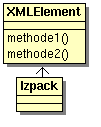
\includegraphics[width=0.15\textwidth]{../image/sol_casInitial.png}
	\hfil
	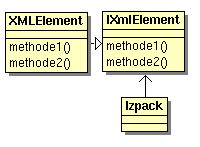
\includegraphics[width=0.3\textwidth]{../image/sol_extractionInterface.png}
	\caption{Extraction de l'interface}
\end{figure}
Nous avons ensuite cree l'implementation de l'adaptateur respectant l'interface. Izpack utilise alors la meme interface mais notre implementation etait utilise. 
\begin{figure}[H]
	\centering
	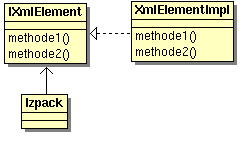
\includegraphics[width=0.4\textwidth]{../image/sol_implementation.png}
	\caption{Implementation de l'adaptateur}
\end{figure}
Il suffit alors de supprimer NanoXml, ses utilisations ayant ete remplace par notre implementation.
\subsection{Fonctionnalites supplementaires}
NanoXml presentait de nombreuses lacunes au niveau respect des standards et fonctionnalites. Cependant, il proposait des fonctionnalites evoluees par rapport a une utilisation standard de Jaxp. Comme ces fonctionnalites etaient utilisees, il nous a fallut les reimplementer.
\subsubsection{Xinclude}
La balise \verb|xinclude| permet d'inclure un fichier xml externe. Ainsi, on peut utiliser un xml très succinct (et donc facilement lisible/compréhensible) qui inclut d'autres fichiers xml decrivant uniquement certaines parties de l'installation. Cette fonctionnalite, absente de nanoXML, avait ete mise en place en modifiant directement le code se son parseur.

Cette fonctionnalite est presente de base dans Jaxp. Il faut pour cela que le parser prenne en compte les namespaces XML. En effet, le Xinclude appartient au namespace xi. Il faut donc utiliser la balise <xi:include/> au lieu de <xinclude/>. Le simple fait de rendre le parser namepaceAware permet d'utiliser la fonctionnalite Xinclude. 

\subsubsection{Xfragment}
La fonctionnalite Xfragment n'est pas presente dans les specifications. Elle permet principalement d'ajouter des elements sans racines avec Xinclude. C'est a dire qu'au contenu du xml a ajouter, on va retirer les noeuds <xfragment>. Par exemple: 
\begin{lstlisting}[language=xml]
<xfragment>
<root1>
	<noeud1>text</noeud1>
</root1>
<root2>
	<noeud1>text</noeud1>
</root2>
</xfragment>
\end{lstlisting}
Si ce xml est rajoute, 2 elements, <root1> et <root2> seront rajoute a l'emplacement du Xinclude. Sans le xfragment, le Xml ne serait pas valide et il y aurait erreur au moment du parse. Le Xfragment agit ici comme conteneur temporaire d'elements.

Cette fonctionnalite a ete rajoute a NanoXml et il etait necessaire de la conserver. Cependant, elle ne fait pas partie des specifications W3C et le parseur n'offrait pas de base cette fonctionnalite. Il a fallut trouver une solution pour assurer la continuite.
\subsubsection{Numero de ligne}
Une fonctionnalite de nanoXML est la gestion des numeros de lignes. Lors qu'une incoherence est detectee dans un xml lu, IzPack previent l'utilisateur de l'erreur, et indique le numero de la ligne responsable dans le xml.

Du point de vue de DOM, les numeros de lignes n'ont pas de signification : une fois le fichier xml parse, seul l'arbre DOM construit en memoire importe. Cet arbre reecrit dans un fichier ne correspondra pas forcement (pour les numeros de lignes, l'indentation, etc) au fichier de depart, sans parler des ajouts/suppressions/modifications de noeuds.

A l'inverse du point de vue de SAX, les numeros de lignes sont obtenues facilement. Dans ce cas la, il est utile de savoir a quel endroit on se trouve dans le document.

Afin d'obtenir les numeros de ligne dans un arbre DOM, les deux points de vue ont ete utilises grace a un Transformer.
On cree une source SAX, a laquelle on ajoute un filtre pour ecouter les evenements (et stocker les numeros de lignes en cas de debut de balise).
En parallele, on cree un resultat DOM, qui contiendra le resultat du parse (l'arbre DOM).
On utilise ensuite un Transformer : il va utiliser la source SAX (les numeros de lignes sont stockees a ce moment par le filtre) et remplir le resultat DOM.
Enfin, il suffit de parcourir l'arbre DOM pour ajouter a chaque element son numero de ligne.
Ce nombre est stocke dans les ``user data'', ajoute dans la version 3  de DOM pour stocker diverses informations supplementaires dans un noeud.
\section{Application et tests}
Une fois la solution realisee, nous l'avons soumis a un certains nombre de tests afin de la verifier.
\subsection{Tests}
Afin d'avoir un comportement le plus fidele possible a celui de nanoXML, de nombreux tests unitaires ont ete ecrits.
\subsubsection{Test unitaires de comparaison}
La solution a d'abord etait elabore de maniere isolee. Le projet contenait notre adaptateur et la librairie NanoXml. Nous avons alors realise une batterie de test couvrant toutes les methodes de l'interface extraites et de tres nombreux cas. Ces tests unitaires effectuent des actions identiques avec notre adaptateur et NanoXML, et compare les resultats. 

Prenons l'exemple de la methode getName(). Le meme fichier Xml est parse par les 2 librairies. Un parcours recursif de l'arbre XML est effectue sur les 2 arbres en memoire. Pour chaque element, on compare le resultat de la methode getName() sur l'element courant. Les retours devant etre toujours egaux.

Comme les methodes de XMLElement sont souvent des recuperations d'informations de la meme nature que getName(), nous avons generalise ce test a ces methodes. Pour cela, une methode se charge de parcourir de maniere recursive l'arbre et d'invoquer la methode testee en comparant leurs resultats. Ceci nous a permit de nous assurer du comportement de l'adaptateur et de deceler des anomalies sur NanoXml.

En couvrant la quasi-totalite des methodes utilises dans IzPack avec de nombreux cas d'utilisation, nous avons pu nous assurer du respect du comportement de notre adaptateur.
\subsubsection{Les tests unitaires sur Xinclude et Xfragment}
Avec l'ajout des fonctionnalites XInclude et XFragment a NanoXml, une batterie de test unitaires a ete fournies. Nous avons donc repris ces tests et nous les avons integres aux tests de l'adaptateurs. 
\subsubsection{Les tests unitaires classiques}
Nous avons crees une batterie de tests unitaires classiques pour notre adaptateur. Ils s'assurent entre autre que le parse, l'exploitation de l'arbre en memoire et l'ecriture du Xml se font correctement.
\subsection{Integration a IzPack}
Une fois la solution realisee, l'integration a IzPack s'est faite de maniere relativement aisee. Sur toutes les utilisations de NanoXml dans Izpack, nous avons utilisee une des classes de notre adaptateur. L'integration s'est faite de maniere relativement aisee et nous avons pu commencer les test sur applications apres.
\subsubsection{Test fonctionnels}
Une phase de test fonctionnels a ete realisee pour tester l'integrite de l'application apres l'integration de notre solution. Ces tests sont des tests manuels sur les installations generes par Izpack. Nous avons donc teste dans un premier temps l'application d'exemple fournit par Izpack. Ces tests ont permis de faire ressortir quelques problemes que nous avons pu regler rapidement.

Suite a cela, nous avons essayer de generer et lancer un installeur plus consequent. Nous avons pour cela utilise l'installeur de Glassfish. La generation et l'installation de glassfish s'est deroule sans probleme.
\subsubsection{Profiling}
Apres la phase d'implementation et de test, nous avons pu commence une phase d'optimisation. En utilisant YourKit, nous avons essaye de detecter les methodes chronophages lors d'une installation et les modifier eventuellements.
\section{Resultats}
Le principal but de notre projet a ete de pouvoir abandonner NanoXml ce qui est chose faite. De plus, l'integration de notre solution a apporte un certain nombres d'avantages.
\subsection{Diminution de la taille des installeurs}
Tout d'abord, l'abandon de NanoXml diminue la taille de IzPack et des installeurs generees comme cette librairies n'a plus a etre embarquees dans les installeurs. NanoXml pese, une fois compile, 116Ko. Notre adaptateur pese 44Ko. Chaque installeur genere par Izpack perdera donc 72Ko. Ce chiffre peut paraitre faible mais portee si l'installeur est telechargee 25000 fois sur un site, presque 1800Mo de bande passante sont economises.
\subsection{Support de fonctionnalitees XML}
Outre le fait d'avoir un parseur plus fiable et recent, un certains nombres de nouveautes ont ete apporte.
\subsubsection{Support de la DTD}
Desormais les DTD (document de validation d'un xml) sont pris en charge.
\subsubsection{Support natif de Xinclude}
De plus, l'inclusion de fichiers xml dans d'autres est supporte nativement, sans avoir a modifier le code du parseur.
\subsection{Integration dans la branche principale}
Regulierement, nous synchronisions notre depot avec la branche principale pour prendre en compte les modifications qui ont ete realisees sur Izpack. Cette synchronisation se passait generalement sans encombre grace a Git excepte quand les modifications concernaient la manipulation de XML et que les fichiers etaient consequent (>3000 lignes).

Cette synchronisation reguliere etait en vue de preparer le merge vers sur la branche principale. Ainsi, une fois notre solution achevee et testee, Julien Ponge a extrait un patch qui a ete soumis a la communaute des developpeurs d'Izpack. Apres quoi, les modifications ont ete portee sur la branche principales et seront disponibles pour la prochaines version d'Izpack, la 4.3.
\section{Au delà du sujet}
Une fois l'objectif du projet atteint, nous avons décidé d'accepter l'offre de Julien Ponge en devenant contributeurs officiels du projet. 
\subsection{Le projet Izpack}
Izpack est une communaute Open-Source, sa structure et son fonctionnement sont particuliers.
\subsubsection{Codehaus}
Le projet est recement passe sous CodeHaus, une fondation dediees au developpement de projets open-source. A ce titre, elle propose un certains nombre d'outils fournis par des sponsors. Par exemple, Atlassian fournit pour les projets leur systeme de suivie de bug, JIRA, JetBrain fournit une license IntelliJ...
\subsubsection{Structure de la communaute}
Les projets sous CodeHaus sont une meritocratie. Un despote supervise un projet. Les developpeurs desirant rejoindre un projet doivent apporter une contribution, montrer leurs motivation et etre approuve par le despote. En general, les decisions se prennent de maniere democratiques pour tout ce qui concernent le projet.

Une mailing-list pour les developpeurs permet de communiquer les informations et prendre les decisions d'un commun accord. Pour eviter tout blocage dans les decisions, le despote a toujours le dernier mot.

Dans le cas de Izpack, le despote est Julien Ponge.
\subsubsection{Système de suivi de bugs, Jira}
L'evolution du projet peut etre suivie via Jira. Les anomalies, lacunes et ameliorations possibles font l'objet d'un ticket. Jira permet alors de suivre et de modifier les tickets avec un workflow est similaire a LightHouse.
\begin{figure}[H]
	\centering
	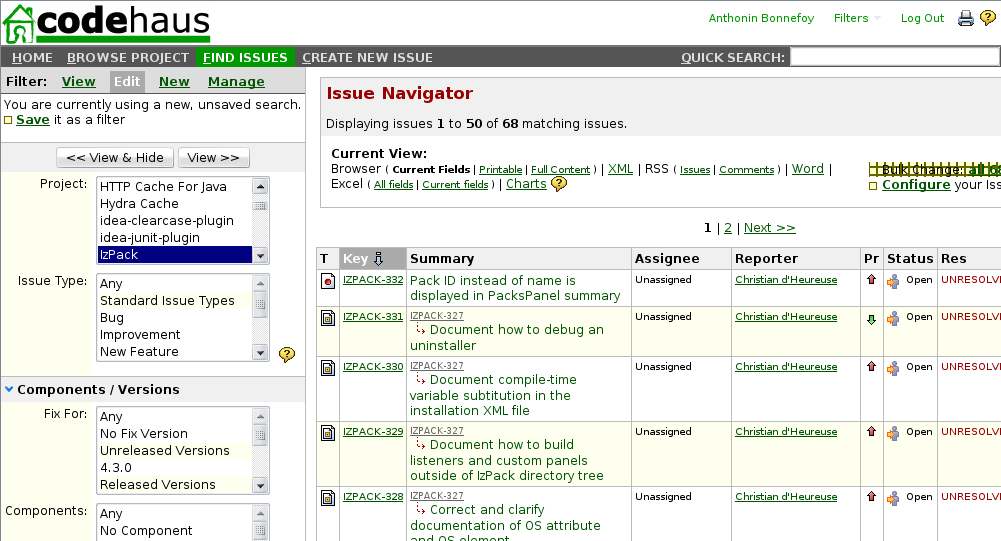
\includegraphics[width=0.8\textwidth]{../image/jira.png}
	\caption{Dashboard Jira}
\end{figure}
\subsection{Suivi de nos apports}
Notre solution etant integree, il est possible que des bugs subsistent dans notre implementation ou une mauvaise interpretation de notre part ne correspond pas au comportement attendus. Le statut de developpeur nous permet de suivre et corriger les problèmes rencontrés par la communauté de IzPack.
\subsubsection{Tests corriges}
Nous avons par exemple corrige des tests unitaires sur les numeros de ligne echouant \cite{IZPACK-306} et sur les conditionsTest \cite{IZPACK-305}.
\subsubsection{Rectification sur une interpretation}
Un probleme est apparu lors de l'utilisation du Xinclude\cite{IZPACK-303}. Ce probleme a ete notifie par un developpeur utilisant la Snapshot et donc ayant recupere nos modifications.

Par defaut, Jaxp resout le chemin de maniere relative au repertoire d'execution et c'est ce qui a ete realisee dans notre implementation. Or, le comportement attendu, plus naturel, est de resoudre le chemin d'inclusion relativement au document incluant le xml.
\subsection{Correction de bugs}
Nous avons egalement corrige plusieurs bugs.
\subsubsection{Probleme lors de l'installation automatique}
Un panel, le TreePacksPanels, ne respectait pas la configuration enregistree lors de l'installation normale.\cite{IZPACK-223}

Un bug cache dans l'installation automatique la faisait quitter silencieusement \cite{IZPACK-309}
\subsubsection{Web installers}
Izpack possede une fonction de creation d'installeurs Web. L'installeur generera des modules qui pourront etre depose sur un serveur web. Cela permet de creer un installeur leger contenant le noyau dur. Les modules aditionnels seront telecharges si ils sont selectionnes.

Cette fonctionnalite presente des lacunes dans la documentation \cite{IZPACK-224} et un bug de fonctionnalite\cite{IZPACK-281}. De plus, il est possible de refactorer la classe utilisee\cite{IZPACK-307}.
\subsubsection{UserInputPanels}
Le panel UserInputPanels doit permettre de decider de l'alignement des elements. C'est a dire qu'il est possible de les placer a gauche, a droite ou au centre \cite{IZPACK-176}. Actuellement, tout les elements sont alignes a gauche. Le travail est en cours de realisation mais les modifications rentrent en concurrence avec le refactoring de dennis.


\subsection{Ameliorations}
% TODO resoudre les bugs jira pour avoir a mettre :p
Outre les corrections de bugs, la qualite du code a ete egalement ameliore. Par exemple, une correction de bug \cite{IZPACK-3xx} a trouve sa correction dans un refactoring de certaines classes, rendant le code plus lisible et portable.

De meme, certaines methodes inutilisees \cite{IZPACK-3xx} (prevues pour des vieilles versions de java) ont pu etre supprimer.